%Farid
\chapter{ PRÉLIMINAIRE DU PROCÉDÉ}
     \section{Représentation et analyse de ensemble (moteur, réducteur, potentiomètre, génératrice        tachymétrique) pour le système $ {S_V}_m \rightarrow V_S$ }
 

\begin{center}
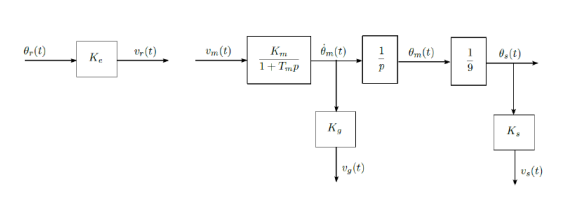
\includegraphics[scale=0.5]{fiiig2.png}
\captionof{figure}{\textit{ Eléments de la platine "asservissement de positon"}}
\label{fig1} 
\end{center}

On considère le système en boucle ouverte l’entrée du système on boucle ouvert est $V_m(t)$ et la sortie mesurée $V_s(t)$, que l’on note  par $ {S_V}_m \rightarrow V_S$.


\subsection{la représentation d’état de ce système, lorsque son vecteur d’état est défni par:}


\begin{equation}
x(t)={(x_1(t),x_2(t))}^T={(V_s(t),V_g(t))}^T
\end{equation}
$x_1=V_s$ et $x_2=V_g$
\\\\


$x_1$=$\frac{K_s}{9p}\frac{x_2}{K_g}$\\\\
$\frac{x_2}{K_g}$=$\frac{K_m}{1+T_m}$
\\
\\

\begin{equation*}
\left\{\begin{matrix}
\dot{x}(t)=Ax(t)+Bu(t)\\ 
y(t)=Cx(t)+Du(t)\\
\end{matrix}\right.
\end{equation*}   

%%%%%%%%%%%comment je vais faire les []%%%%%%%%%
$\dot{X}$=$\begin{bmatrix}0&\frac{K_s}{9K_g}\\0&-\frac{1}{T_m}\end{bmatrix}x$
\quad+\quad $\begin{bmatrix}0\\
\frac{K_mK_g}{T_m}
\end{bmatrix}V_m
$
\\\\

avec U=Vm , Y=Vs, X est le vecteur d'état\\
D'où: Il n y a  pas de transfert direct en boucle ouvert car D=0\\
alors: $$y=[1\quad0].X$$ 



\subsection{Détermination des pont d’équilibre lorsque $v_m$(t) est constante, et L’étude de stabilité }

\begin{center}
$\dot{X}_eq=0$
\end{center}

\begin{center}
$x_2=0 $\\
$x_2=K_g.K_m.V_m$ \\
\end{center}

\begin{center}
si $V_m$ $\ne $0 donc il n y a pas de point d'équilibre \\
si $V_m$=0 alors\\
 $\dot{X}_eq=$ \end{center}$$\begin{pmatrix} 0\\\alpha \end{pmatrix}$$
 
 \begin{center}
avec $\alpha$ $\in$ R
\end{center}

\textbf{Étude de la stabilité du système}\\
On utilisant  la commande Matlab eig(A),on voie que le système est stable mais asymptotiquement parlent n'est pas stable, ce que nous as permet de dir que le système  est stable c'est les valeur propre:  
$$\begin{matrix}
0\quad-3,33
\end{matrix}$$
\textbf{Ce qu nous amène a dir on deux mode qui sont $e^{-3.33t}$ et 0}\\
On as donc deux mode un mode  convergent et un mode stationnaire.\\

\textbf{Etude de la commandabilité et l'observabilité}\\
On peut dire qu’un système est commandable   d’âpres   le critère de Kalman si et seulement si les vecteurs [B], [A]*[B]sont linéairement indépendants.\\
On doit avoir le rang de matrice de commandabilité  rang=2, est comme ces condition sont vérifie donc le système est commandable.
Est pour l'observabilité on le rang de la matrice d'observabilité =2, alors le système est observable.

\subsection{Représentations sous forme  compagnes de commande et d'observation}

\textbf{Le système}
\\

$A$=
$\begin{bmatrix} 
0 & 10.5820 \\
0 & -3.3333
\end{bmatrix}
$





$B$=
$\begin{bmatrix} 
0 \\
2.4500  
\end{bmatrix}
$\\


$C$=
$\begin{bmatrix} 
1 & 0 
\end{bmatrix}$
\\\\\\
$D$=$[0]$
\\\\

\textbf{Matrice de passage de commandabilité est}
 

$$ 
P_c = (AB + (1/Tm)B \quad B)
$$
$P_c$=$\begin{bmatrix}
\frac{K_sK_m}{9T_m}&0\\
0&\frac{K_mK_g}{T_m}
\end{bmatrix}$
\\\\

\textbf{Représentation sous forme Compagne de commande:}\\

$A_c$=
$\begin{bmatrix} 
0 & 1 \\
0 & -3.333
\end{bmatrix}$
\quad
$B_c$=$
\begin{bmatrix} 
0 \\
1  
\end{bmatrix}
$
\quad
$C_c$=
$\begin{bmatrix} 
0.3889 &0 
\end{bmatrix}$
\quad
$D_c$=[0]
\\\\

\textbf{Matrice de passage de observabilité est}\\


$P_o$ =$
\begin{bmatrix}
(CA + (1/Tm)C\\ C
\end{bmatrix}$
\\

$P_o^1$=$\begin{bmatrix}
-\frac{1}{T_m}&\frac{K_s}{9K_g}\\
1&0
\end{bmatrix}$
\\\\

\textbf{Représentation sous forme compagne d'observation:}\\

$A_o$=
$\begin{bmatrix} 
0 & 0 \\
1 & -3.333
\end{bmatrix}$
\quad
$B_o$=
$\begin{bmatrix} 
0.3889 \\
0  
\end{bmatrix}$
$$
$$
$C_o$=
$\begin{bmatrix} 
0 & 1 
\end{bmatrix}$
\quad
$D_c$=[0]

\section{Représentation et analyse de l’ensemble (moteur, réducteur, potentiomètre, génératrice
tachymétrique) pour le système }
\subsubsection{La représentation d’état de ce système en conservant la définition du vecteur d’état }


$A$=
$\begin{bmatrix} 
0 & 10.5820 \\
0 & -3.3333
\end{bmatrix}$
\quad
$B$=
$\begin{bmatrix} 
0 \\
2.4500  
\end{bmatrix}$
\quad
$C$=
$\begin{bmatrix} 
0 & 1 
\end{bmatrix}$
\quad
$D$=[0]

\subsubsection{Étude de stabilité, observabilité, observabilité}
après avoir  simuler sous Matlab on voie que une valeur propre  n'est pas négative ($\lambda=0$)ce qui nous amène a dir que le système n'est pas stable asymptotique, mais on peut placer nos valeur propre là on veut car le rang de la matrice de commandabilité=2 qui est égale aussi ou nombre de valeur propre, mais d'autre part le rang de la matrice d’observabilité =1<2  alors notre système n'est pas observable depuis    
$V_g$.